\documentclass[a4paper, 12pt, oneside]{article}


% idioma
\usepackage[utf8]{inputenc}
\usepackage[spanish]{babel}

%tablas
\usepackage{booktabs}

%rotar tablas
\usepackage{rotating}

%color tablas
\usepackage{colortbl}



%espaciado
\usepackage{setspace}
\onehalfspacing
\setlength{\parindent}{0pt}
\setlength{\parskip}{2.0ex plus0.5ex minus0.2ex}


%margenes según n. icontec
\usepackage{vmargin}
\setmarginsrb           { 4.0cm}  % left margin
                        { 3.0cm}  % top margcm
                        { 2.0cm}  % right margcm
                        { 2.0cm}  % bottom margcm
                        {   0pt}  % head height
                        {0.0 cm}  % head sep
                        {   9pt}  % foot height
                        { 1.0cm}  % foot sep

% inserción url's notas de pie.
\usepackage{url}

%otras
\usepackage{verbatim}

% Paquetes de la AMS:
\usepackage{amsmath, amsthm, amsfonts}
\addto\captionsspanish{\def\refname{\textsc{Bibliografía}}}

\newcommand\portada{
	\begin{titlepage}
		\begin{center}
			{\large \bf ESTUDIO DE MERCADO DEL PROYECTO }
			\vfill
% 			{\large\bf PRESENTADO POR \par}
			{\large\bf SEBASTIÁN GÓMEZ GONZÁLEZ \par}
			{\large\bf SANTIAGO GUTIERREZ ALZATE \par}
			\vfill
			{\large\bf UNIVERSIDAD TECNOLÓGICA DE PEREIRA  \par}
			{\large\bf FACULTAD DE INGENIERÍAS \par}
			{\large\bf INGENIERÍA DE SISTEMAS Y COMPUTACIÓN \par}
			{\large\bf PEREIRA\par}
			{\large\bf SEPTIEMBRE DE 2010 \par}
		\end{center}
	\end{titlepage}
}


\begin{document}
\portada

	\tableofcontents
	\clearpage
	
	\begin{center}
	\section{Formulación del problema}
	\end{center}

	Los problemas visuales afectan a una gran parte de la población, tanto en Colombia\footnote{Según el DANE en su gran censo nacional realizado en el año 2005, se estima que el 6.3\% de la población colombiana sufre de alguna discapacidad. De estas personas con discapacidad se estima que el 43.4\% tienen dificultades para ver aun con lentes.} como a nivel mundial\footnote{La organización mundial de la salud estima que en el mundo hay 161 millones de personas con problemas visuales, de los cuales 37 millones son ciegos.}, estos traen consigo consecuencias devastadoras para las personas que los sufren, afectando su calidad de vida significativamente. Entre todos los problemas que sufren las personas con discapacidades visuales, uno de los más críticos es el del acceso a la información; esto debido a que la mayoría de la información los seres humanos reciben del entorno llega a través de los ojos. Los problemas para obtener información causan que las personas con discapacidades visuales se queden rezagadas con respecto a los demás miembros de la sociedad, impidiendo así que tengan las mismas oportunidades de vida que una persona con sus cinco sentidos intactos. Generalmente, esto causa un efecto de exclusión y de segregación en estas personas debido a que son vistas como una carga, tanto por si mismas como por las personas que los rodean. 

	A partir de la incidencia del problema, una forma de ayudar a que las personas con discapacidades visuales tengan una mejor calidad de vida es lograr que puedan tener acceso a la información que se encuentra en documentos escritos, tales como cartas, libros, y volantes. Esto puede ser logrado a través un sistema de reconocimiento óptico de caracteres que reconozca el texto escrito en estos documentos y le lea a la persona invidente lo que dicen. Sin embargo, para que sea una solución efectiva al problema, se requiere de un sistema que le permita a los discapacitados visuales acceder a la información escrita de una manera rápida y fácil, lo cual implica gran movilidad. Si bien existen múltiples sistemas de reconocimiento óptico de caracteres para computadores de escritorio, estos no poseen dicha movilidad, porque además del computador, también necesitan de un escáner para funcionar. Así pues, para que un sistema de este tipo pueda ser utilizado en múltiples lugares, se requiere de algún dispositivo que sea: pequeño, fácilmente transportable y capaz de hacer el trabajo en un tiempo razonable. Los teléfonos inteligentes parecen ser una buena alternativa, no obstante, existen grandes diferencias entre un computador de escritorio y un teléfono inteligente, entre ellas se pueden resaltar las siguientes:
	
	\begin{itemize}
	
	\item La memoria y la capacidad de procesamiento son muy reducidas en los teléfonos inteligentes con respecto a los computadores de escritorio.

	\item El tamaño de la memoria cache es mucho más pequeño en los teléfonos inteligentes. Como resultado de esto, los algoritmos diseñados para computadores de escritorio pueden ser muy lentos en los teléfonos inteligentes, pues se hicieron pensando en caches de varios mega-bytes.

	\item Un computador de escritorio normalmente tiene instaladas múltiples librerías de propósito general que son utilizadas por distintos programas, un teléfono inteligente, en cambio, solo provee las librerías más básicas.

	\end{itemize}

	La diferencia mas importante, sin embargo, es que en los computadores de escritorio las imágenes son obtenidas por medio de un escáner, logrando condiciones de iluminación muy buenas y uniformes, mientras en los teléfonos inteligentes las imágenes se obtienen por medio de una cámara fotográfica. Esta diferencia es muy importante para el reconocimiento óptico de caracteres, en especial si quien toma la foto es una persona invidente, ya que en este caso diversas variables como la inclinación del texto, la iluminación no uniforme, y las deformaciones elásticas del texto debido a la forma del papel en reposo, cobran más relevancia, pues la persona invidente podría tomar la fotografía inclinada, en el sentido contrario, o en un lugar con poca luminosidad.

	Para dar solución al problema de limitación en la capacidad de procesamiento de los teléfonos inteligentes se puede utilizar una de sus grandes ventajas: son por naturaleza dispositivos de alta conectividad. Cada vez los planes de telefonía son mas económicos y hay mas disponibilidad de redes inalámbricas, a las cuales los teléfonos inteligentes tienen acceso, en diferentes sitios públicos como institutos educativos y bibliotecas. Esta alta conectividad posibilita la construcción de un sistema de reconocimiento óptico de caracteres con una arquitectura cliente-servidor, en la cual el teléfono inteligente pueda enviar la imagen por internet y esta sea procesada por un servidor con una capacidad de computo mucho mayor. Este sistema tendrá las mismas ventajas de movilidad y rapidez deseadas. La capacidad de procesamiento de los celulares inteligentes también ha incrementado en los últimos años, lo que permitiría hacer parte del procesamiento en el celular, con el objetivo de reducir el ancho de banda requerido para enviar la imagen al servidor y por tanto el costo.

	Para solucionar los problemas asociados con la inclinación del texto que se puede producir en las imágenes tomadas por la persona invidente, se hace necesario un sistema de reconocimiento óptico de caracteres que pueda reconocer exitosamente fotos tomadas con distintos grados de inclinación o incluso en el sentido contrario.

	Después de una búsqueda en más de 20 artículos científicos relacionados al tema de reconocimiento óptico de caracteres, y de revisar la documentación técnica de varios OCRs libres, no se encontró un sistema de reconocimiento de caracteres por un medio óptico que haya sido desarrollado para ser usado por personas invidentes en teléfonos inteligentes, que sea de código libre y abierto, y que solucione los problemas de inclinación y luminosidad antes presentados. 	
	
	\clearpage

	\begin{center}
	\section{Justificación}
	\end{center}
	
	Además de esto, un sistema móvil para reconocer texto de documentos impresos presentaría los siguientes beneficios respecto de los sistemas tradicionales como las impresoras braille y los lectores basados en escáner:

	\begin{itemize} 

	\item Un menor costo, al no ser necesario adquirir un computador de escritorio, escáner o impresora braille.

	\item Portabilidad: ninguno de los sistemas tradicionales esta diseñado para ser llevado en todo momento por el usuario, dificultando el acceso al conocimiento e información que no se encuentre en el lugar físico en el que se encuentra alguno de estos sistemas.
	
	\item Una solución económica que pueda ejecutarse en un dispositivo móvil, sin necesidad de hardware adicional, haría posible que cada invidente pudiera tener su propio sistema de OCR personal, mientras que los otros sistemas usualmente (por su costo) son adquiridos por instituciones en cantidad limitada.

	\item Aportar al conocimiento: Al desarrollar este aplicativo se tendrán que hacer pruebas experimentales cuyos resultados aporten a otras investigaciones.
	\end{itemize}
	\clearpage

	\begin{center}
	\section{Misión, Visión, Objetivos y Metas}
	\end{center}
	
	\subsection{Misión}
	Ser una empresa líder en la asistencia tecnológica a las personas invidentes, brindándoles
	soluciones que les permitan integrarse a la sociedad usando tecnologías
	de la información y de comunicaciones.
	
	\subsection{Visión}
	Ser una empresa mundialmente reconocida en la investigación y desarrollo de aplicativos y servicios
	para móviles, relacionados con procesamiento de imágenes y visión por computador enfocada a la 
	asistencia a las personas invidentes.
	
	\subsection{Objetivo general}
	Desarrollar un sistema que usando un teléfono inteligente, le permita a las personas invidentes acceder
	a textos impresos tomándole una foto a estos textos. Este sistema le prestará el servicio de convertir
	la imagen a texto a los usuarios invidentes y sus teléfonos convertirán el texto a voz.
	
	\subsection{Objetivos específicos}
	\begin{itemize}
	\item Realizar un estudio de mercado, técnico y financiero de la idea de proyecto.
	\item Realizar una investigación científica de los algoritmos y técnicas para llevar a cabo este proyecto.
	\item Diseñar e implementar una aplicación con las especificaciones antes mencionadas.
	\item Buscar financiamiento en varias instituciones para proyectos de emprendimiento y
	 de impacto social.
	\item Buscar convenios con empresas prestadoras de servicios de celulares y con las instituciones
	 para personas invidentes en cada país para iniciar la implantación del servicio en el mercado.
	\end{itemize}
	
	\subsection{Metas}
	\begin{itemize}
	\item Realizar un estudio de mercado, técnico y financiero de la idea de proyecto usando
		como plazo no mas de 6 meses.
	\item Realizar una investigación científica de los algoritmos y técnicas para llevar a cabo este proyecto,
		escribir artículos de las investigaciones, revisando cada dos meses los avances y resultados de la
		investigación.
	\item Diseñar e implementar una aplicación con las especificaciones antes mencionadas, en los plazos
	definidos en la etapa de investigación.
	\item Buscar financiamiento en varias instituciones para proyectos de emprendimiento y
	 de impacto social, a las que se puedan aplicar y en los plazos establecidos por cada uno de estos
	 programas de financiamiento.
	\item Buscar convenios con empresas prestadoras de servicios de celulares ofreciendo el servicio
	 y los clientes por un determinado porcentaje de el plan tomado por la persona invidente. Primero
	 se hablará con las compañías celulares de Colombia y con el INCI (Instituto nacional para ciegos).
	\end{itemize}
	
	\clearpage
	\begin{center}
	\section{Indicadores}
	\end{center}
	
	\subsection{Indicadores de monitoréo}
	\begin{itemize}
		\item {\bf Velocidad de desarrollo}($M_1$): Para medir el avance de desarrollo se tomarán la cantidad
			de líneas de código $l$ y se dividirán entre el tiempo que ha transcurrido $t$.
			\[M_1 = \frac{l}{t}\]
		\item {\bf Avance de desarrollo}($M_2$): Para medir el avance de desarrollo se tomarán la cantidad
			de casos de uso terminados $C_f$ y se dividirán entre la cantidad de casos de uso que se deberían
			llevar $C_p$.
			\[M_2 = \frac{C_f}{C_p}\]
		\item {\bf Efectividad del aplicativo}($M_3$): Se define efectividad como la cantidad de caracteres(Letras)
			que se leen exitosamente a la persona invidente. Si $L_c$ son las letras leídas exitosamente y $L_t$
			son el total de letras entonces:
			\[M_3 = \frac{L_c}{L_t}\]	
		\item {\bf Búsqueda de financiamiento}($M_4$): Este es un indicador para comparar la cantidad adicional de
			financiamiento recibida por unidad de tiempo. Si $\Delta f$ es la cantidad de dinero adicional recibida
			y $\Delta t$ es la cantidad de tiempo en la que se recibió este financiamiento, entonces:
			\[M_4 = \frac{\Delta f}{\Delta t}\]
	\end{itemize}
	
	\subsection{Indicadores de impacto}

	\begin{itemize}
		\item {\bf Personas beneficiadas}($I_1$): Cantidad de personas beneficiadas $P_b$ sobre el total
			de personas afectadas por el problema (Personas invidentes) $P_i$.
			\[I_1 = \frac{P_b}{P_i}\]
		\item {\bf Reconocimiento}($I_2$): Una manera indirecta de medir el reconocimiento del proyecto por su
		 finalidad social es por la cantidad de premios $P$ que otorgados por este fin. Aunque solo sería útil
		 al principio.
			\[I_2 = \frac{P}{\Delta t}\]
		\item {\bf Calidad de vida de los usuarios}($I_3,I_4$): Al terminar el proyecto para ser usado comercialmente,
			se podrían hacer encuestas que ayuden a medir el mejoramiento de la calidad de vida de los usuarios.
			Si $S$ es el promedio de los salarios de los usuarios, un primer indicador que mida el aumento porcentual
			en sus salarios podría ser:
			\[I_3 = \frac{\Delta S}{S}\]
			Si $F$ es el promedio de una medida subjetiva de su nivel de felicidad, otro posible indicador sería:
			\[I_4 = \frac{\Delta F}{F}\]
	\end{itemize}
	
	\subsection{Indicadores de resultado}
	\begin{itemize}
		\item {\bf Costo/Beneficio monetario del proyecto}($R_1$): Si la cantidad de personas horas hombre $H$,
			el costo promedio de la hora $C_h$, y el nivel de ingresos de los $N$ beneficiarios aumenta en
			$I_3$(Ver definición en indicadores de impacto) puntos porcentuales. Se calcularía:
			\[R_1 = \frac{N \times I_3 \times S}{H \times C_h}\]
			E indicaría cuanto aumentaron los ingresos en general de los usuarios por cada peso invertido
			al proyecto.
		\item {\bf Crecimiento empresarial}($R_2$): Si en un periodo de tiempo $t$, entran unos ingresos $I$ y
			se tienen unos gastos $C$; Este indicador se da por:
			\[R_2 = \frac{I-C}{t}\]
		\item {\bf Incremento de usuarios}($R_3$): Si N es el número de usuarios, este indicador se calcularía:
			\[R_3 = \frac{\Delta N}{N}\]
			E indicaría un incremento porcentual de los usuarios del servicio.
	\end{itemize}
	\clearpage
	
	\begin{center}
	\section{Contextualización del proyecto}
	\end{center}
	
	\subsection{Relación con el plan de competitividad}
	La relación del proyecto con el plan regional de competitividad se puede ver el cuadro \ref{regional}. Note
	que los principales programas a los que el proyecto está relacionado tienen que ver con la investigación,
	ciencia, tecnología y creación de empresa. Estos son importantes para que la región crezca, y ya que toda
	región tiene sectores en los que es mas competente, Risaralda gracias a la Universidad tecnológica y a
	ParqueSoft ha mostrado que tiene un gran potencial en sectores de la informática y tecnología.
	
	\begin{sidewaystable}[h]	
		\caption{Relación del proyecto con el plan de competitividad}
		\begin{tabular}{ | p{4cm} | p{4cm} | p{14cm} | }
		\hline
		Objetivos & Proyecto priorizado & Fundamentación\\
		\hline					
		Innovación, investigación, ciencia y tecnología & Red de Nodos de Innovación, ciencia y tecnología & Los spin off y los spin offs universitarios son mencionados en el plan de competitividad de Risaralda como variables importantes en este objetivo, nuestro proyecto, que se desprende del proyecto de grado y es por tanto un spin off universitario, es un proyecto de investigación en el área de visión e inteligencia artificial. Ya que este tipo de software es muy nuevo, e incluso inexistente en nuestro país, seria un producto innovador en nuestra región. \\
		\hline
		Emprendimiento y desarrollo empresarial & Programa de emprendimiento y empresarismo & La creación de empleo es parte fundamental del plan de competitividad de Risaralda, nuestra proyecto, que empieza como un emprendimiento, puede brindar oportunidad de empleo a muchas personas de la región que se interesen en el campo de la inteligencia artificial y el reconocimiento de patrones. El proyecto también comprende la creación de una empresa dedicada al área de inteligencia artificial, algo acorde con este objetivo regional. \\
		\hline
		Fortalecimiento de sectores estratégicos & Ciudad digital y gobierno en línea & Ya que el sector de las tecnologías de la información y las comunicaciones es un sector priorizado en el plan de competitividad, nuestro proyecto, que involucra tanto información como el área de comunicaciones, puede hacer un aporte interesante a este sector. Así mismo, el programa gobierno en línea establece que debe haber una gran accesibilidad para posibilitar el acceso a la información a las personas invidentes, nuestro proyecto comparte este propósito y podría expandirlo para incluir también gran cantidad de documentos impresos que aun no se han digitalizado. \\
		\hline
		\end{tabular}
		\label{regional}
	\end{sidewaystable}

	\subsection{Relación con los planes del país}
	En el cuadro \ref{nacional} se muestra como el proyecto tiene también relación con los planes de
	la ciudad, del departamento y del país. Cabe destacar que este proyecto también tiene una
	fuerte relación con las metas del milenio establecidas por la organización de las naciones
	unidas (ONU).
	
	\begin{sidewaystable}[h]
		\caption{Relación del proyecto con los planes del país}
		\begin{tabular}{ | p{3cm} | p{8cm} | p{3cm} | p{3cm} | p{6cm} | }
		\hline
		Plan & Objetivo & Programa & Proyecto & Fundamentación \\
		\hline					
		Plan de Desarrollo Municipal Pereira “Región de Oportunidades” 2.007-2011 & “Cambiar las causas que generan las inequidades y retrasan el mejoramiento en las condiciones de vida de las personas, avanzando hacia un sistema complementario de asistencia pública integral y responsable con la generación de oportunidades para el desarrollo autónomo, bajo un esquema de corresponsabilidad social, armonizado con los compromiso de la humanidad en las metas del milenio, la visión Colombia 2019, el Plan Nacional de Desarrollo y el Programa de Gobierno avalado por la ciudadanía de Pereira en el voto de confianza asignado a la presente administración.” & Programa población prioritaria & Proyecto “Atención Sin Distinción” & Este proyecto involucra “atención a la población con limitaciones para ver, para caminar, para oír, para entender aprender, etc", lo que significa que la atención a las personas invidentes es uno de sus objetivos, nuestro proyecto es acorde con dicho objetivo. \\
		\hline
		Plan de Desarrollo Departamental “Risaralda Sentimiento de Todos” & "Los Ocho Objetivos del Milenio establecidos en los convenios internacionales y ratificados por Colombia, porque ningún grupo social podrá alcanzar metas mínimas de desarrollo humano sostenible sin acceso a servicios de educación, salud, seguridad alimentaria, recreación, vivienda digna, agua potable y saneamiento básico, salud ambiental y mejoramiento del ingreso, entre otros factores" & Línea Estratégica Equidad e Inclusión Social & Programa: La escuela un lugar para todos & Dado que una de las grandes dificultades para las personas invidentes a la hora de estudiar es el acceso a la información, nuestro proyecto puede ayudar a que estas personas accedan a la información escrita, que en muchos casos es la única información disponible, especialmente en los colegios de los municipios menos desarrollados. \\
		\hline
		Plan de Desarrollo Nacional 2.010-2014 "Prosperidad para Todos" & "Ser un país con prosperidad para todos: con más empleo, menor pobreza y más seguridad." & Formación de capital humano & Calidad en la formación impartida por el sistema educativo colombiano & La calidad de la educación depende del nivel de acceso a la información de quienes la reciben, nuestro proyecto busca facilitar este acceso a las personas invidentes. \\
		\hline
		\end{tabular}
		\label{nacional}
	\end{sidewaystable}
	
	\subsection{Relación sistemas de información}

	Nuestro proyecto se relaciona con SIPER, Sistema de información para el emprendimiento en Risaralda, ya que precisamente es un emprendimiento y por tanto este sistema de información nos puede ser útil para conectarnos con emprendimientos relacionados.

	\subsection{Relación área metropolitana}

	Nuestro proyecto se puede relacionar con el proyecto de emprendimiento del área metropolitana, por que ambos tienen que ver con emprendimiento en las universidades.

	\clearpage
	
	\begin{center}
	\section{Estudio de mercado}
	\end{center}
	%\subsection{Objetivo}
		
	\subsection{Submercados}
	Para este estudio se analizaran los 5 submercados: proveedores, competidores, distribuidor, consumidor y el submercado externo. Los submercados se analizaran en los siguientes puntos del estudio de mercado.	

	\subsection{Análisis histórico, situación vigente y proyectada}
	Para el análisis en retrospectiva, prospectiva y perspectiva se utilizaron tablas. Cada una de estas tablas hace el análisis de los 5 submercados. El submercado de proveedores se puede ver en la tabla \ref{provHistorico}, el de competidores en la tabla \ref{compHistorico}, el de distribuidores en la tabla \ref{distHistorico}, el de consumidores en la tabla \ref{consHistorico} y el externo en la tabla \ref{extHistorico}.
	
	\subsection{Consumidores}
	Para el proyecto, se plantea que se pueden tener líneas para clientes institucionales y para individuales:

	\subsubsection{Clientes Institucionales}
	A corto plazo, el mercado de clientes institucionales es el mas llamativo. Instituciones como el INCI en Colombia y la ONCE en España, tienen recursos para invertir en tecnología de asistencia a personas invidentes. Una ventaja adicional que tiene atender a este mercado, es que los usuarios de los servicios de estas instituciones, al conocer el servicio prestado por la empresa, pueden adquirir este servicio como individuos. Así, al atender a este mercado se podría abrir el mercado de clientes individuales.

	\subsubsection{Clientes individuales}
	Este mercado es difícil de abrir al corto plazo, pero al ser muchas mas personas las usuarias del servicio se convierten en un mercado muy prometedor. Además, no solo hay que limitarse al mercado nacional, y la tendencia en el mundo ha mostrado que las personas invidentes se integran cada vez mas a la sociedad.	
	
	\begin{table}
		\caption{Análisis histórico, situación vigente en el submercado de proveedores}
		\begin{tabular}{ | p{4cm} | p{10cm} | }
		\hline
		Situación & Análisis \\
		\hline					
		Análisis histórico & 
		Haciendo un análisis en retrospectiva, hace unos 20 años los proveedores de equipos de cómputo para atender múltiples usuarios eran muy pocos, vendían sus equipos a costos muy elevados y la mayoría no tenían oficinas en el país. Por tanto los costos de los equipos era mucho mas elevado, además de los costos y riesgos de información, y la falta de personal técnico que pudiera utilizar esos equipos y prestarles el debido mantenimiento. \\
		\hline
		Situación Vigente &
		En la actualidad, la cantidad de proveedores de equipos ha aumentado y han bajado los precios para llegar a los mercados de la pequeña y mediana empresa. Dado que el mercado (compradores y proveedores) de equipos es mas grande, hay empresas locales que importan grandes cantidades de equipos, teniendo menos costos, mas técnicos especializados y mejor servicio. \\
		\hline
		Situación proyectada &
		La tendencia es que cada vez es mas fácil conseguir equipos y son mas económicos. Esto plantea un escenario próspero en cuanto a la disponibilidad de los recursos materiales necesarios para el desarrollo del proyecto. Hablando cuantitativamente, la ley de Moore establece que cada 3 años de duplica la capacidad de los equipos de cómputo (cabe anotar que Moore es ejecutivo de la compañía multinacional Intel, y que su ley se ha mantenido hasta el momento). \\
		\hline
		\end{tabular}
		\label{provHistorico}
	\end{table}
	
	\begin{table}
		\caption{Análisis histórico, situación vigente en el submercado de competidores}
		\begin{tabular}{ | p{4cm} | p{10cm} | }
		\hline
		Situación & Análisis \\
		\hline					
		Análisis histórico & 
		En el pasado, la única forma que tenían las personas invidentes era a través del texto en Braille. El Braille es un código para textos impresos que se basa en el alto relieve de los caracteres. \\
		\hline
		Situación Vigente &
		En la actualidad, existen productos tecnológicos que pueden competir con nuestro producto. Entre estos productos de encuentran las impresoras y pantallas Braille dinámicas, lectores de pantalla de computadores y lectores de texto basados en computador de escritorio utilizando Scanner. Aunque el director nacional del INCI (Instituto Nacional de Ciegos), ha confirmado que en el país no existe ningún sistema de este tipo para dispositivos móviles. \\
		\hline
		Situación proyectada &
		En un futuro cercano no se ven evidencias de que nuevas empresas quieran entrar a competir en nuestro servicio, al menos a nivel nacional. De hecho en la actualidad los competidores no son empresas nacionales, y sus clientes son instituciones y no personas individuales. (Fuente, Director del INCI)\\
		\hline
		\end{tabular}
		\label{compHistorico}
	\end{table}
	
	\begin{table}
		\caption{Análisis histórico, situación vigente en el submercado de distribuidores}
		\begin{tabular}{ | p{4cm} | p{10cm} | }
		\hline
		Situación & Análisis \\
		\hline					
		Análisis histórico & 
		El primer celular comercial fue lanzado en el año de 1979 en Japón, a partir de ese momento el uso de celulares se empezó a masificar poco a poco. Sin embargo, los celulares tuvieron una mayor penetración en las ciudades y áreas desarrolladas, en las áreas rurales la penetración siempre fue mucho menor.
		\\
		\hline
		Situación vigente &
		Hoy en día los celulares son ubicuos en los países desarrollados, e incluso en el mundo la penetración es del 75\%. Esto puede ser apreciado en la figura \ref{fig:usocel1}.
		Sin embargo los celulares inteligentes (smartphones) todavía no son muy utilizados, pues solo aproximadamente 200 millones de personas los utilizan.
		 \\
		\hline
		Situación proyectada &
		Se espera que el mercado de los celulares continúe hasta el punto que prácticamente todos los habitantes del planeta posean un celular. La tendencia de los celulares
		inteligentes es a masificarse, es por ello que las compañías de tecnología más grandes del mundo están promocionándolos mucho, incluso de una manera no justificada
		por la demanda actual, por cuanto esperan que este sector les de muchas ganancias en el futuro.
		 \\
		\hline
		\end{tabular}
		\label{distHistorico}
	\end{table}

	\begin{figure}[htb]
	\begin{center}
	\leavevmode
	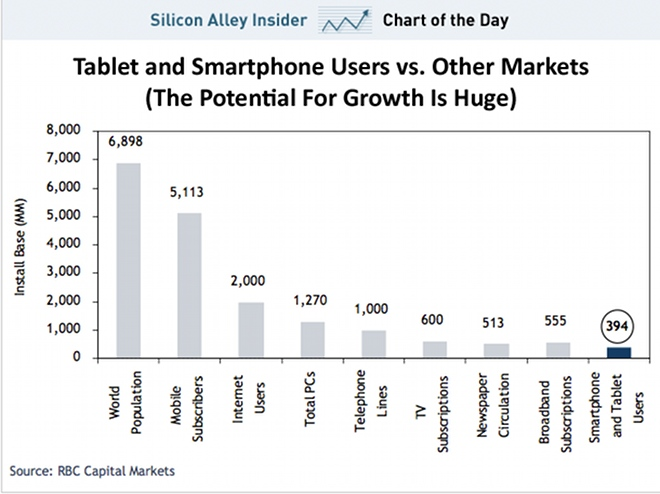
\includegraphics[width=7cm]{img/usocel1.jpg}
	\end{center}
	\caption{Uso de los celulares a nivel mundial}
	\label{fig:usocel1}
	\end{figure}
	
	\begin{table}
		\caption{Análisis histórico, situación vigente en el submercado de consumidores}
		\begin{tabular}{ | p{4cm} | p{10cm} | }
		\hline
		Situación & Análisis \\
		\hline					
		Análisis histórico & 
		En el pasado las personas invidentes se rezagaban del resto de la sociedad, dado que no podían desempeñar las mismas labores y escribir de la misma forma que el resto de las personas. La sociedad tampoco les brindaba oportunidades a las personas invidentes. \\
		\hline
		Situación Vigente &
		El nivel de oportunidades para las personas invidentes ha mejorado, la legislación colombiana proteje el derecho a la igualdad de las personas con discapacidades brindándoles ventajas. En muchos casos, el gobierno ofrece beneficios a las empresas que contraten personas con discapacidades y se aumenta la inclusión en la sociedad; aunque la diferencia de oportunidades es aun alta con respecto al resto de la sociedad. Las instituciones como el INCI, han adquirido tecnologías que les permita a las personas invidentes tener acceso a los documentos escritos en texto común. \\
		\hline
		Situación proyectada &
		Las personas invidentes se van a vincular cada vez mas en la sociedad, y necesitarán tecnología que les permita leer documentos en formatos legibles por el resto de las personas. También crecerá la tendencia de el nivel de educación alcanzado por las personas invidentes y las instituciones educativas necesitarán también esta tecnología, como ha mostrado la tendencia hasta el momento en el INCI.
		 \\
		\hline
		\end{tabular}
		\label{consHistorico}
	\end{table}
	
	\begin{table}
		\caption{Análisis histórico, situación vigente en el submercado externo}
		\begin{tabular}{ | p{4cm} | p{10cm} | }
		\hline
		Situación & Análisis \\
		\hline					
		Análisis histórico & 
		En el mercado externo, muchos gobiernos en el pasado han dado beneficios a las personas invidentes que les ha permitido tener recursos para hacer sus propias compras. Como un ejemplo particular, a la ONCE (Organización Nacional de Ciegos de España) se la adjudico una lotería. \\
		\hline
		Situación Vigente &
		Algunas compañías extranjeras se dedican a producir soluciones para personas invidentes, y no solamente compañías de tecnología, pero que cuentan con gran apoyo de los estados. Por ejemplo hay compañías dedicadas a entrenar perros para asistir a las personas invidentes, y el entrenamiento de estos animales es muy costoso dado que se necesita personal altamente capacitado; ya que la persona invidente le confía la vida al animal y por tanto se tiene una gran responsabilidad. \\
		\hline
		Situación proyectada &
		Se espera que la tendencia en el exterior continúe, así como se espera que incremente la demanda al darle mayores recursos a las asociaciones de personas invidentes, también se espera que incremente la oferta de servicios para este grupo poblacional. \\
		\hline
		\end{tabular}
		\label{extHistorico}
	\end{table}
		
	\subsection{Estrategia comercial}
	 
	\subsubsection{Producto}
	El producto que se va a ofrecer es en realidad un servicio de reconocimiento óptico de caracteres para personas invidentes. Este servicio incluye una aplicación para distintos
	sistemas operativos de teléfonos móviles, la cual no tendrá costo, pues se cobrara el servicio.

	\subsubsection{Precio}
	Para determinar el precio se va a hacer una encuesta que permita establecer los parámetros A1-A4, Y, Pb, Pub, de la siguiente ecuación:

	\begin{equation}
	Q = A1 \times P + A2 \times Y + A3 \times Pb + A4 \times Pub 
	\end{equation}

	Donde:

	\begin{itemize}
	      \item $Q$ : cantidad demandada en el periodo
	      \item $A1 A4$ : parámetros de la demanda
	      \item $Y$ : ingresos per capita
	      \item $Pb$ : población
	      \item $Pub$ : publicidad
	      \item $P$ : precio
	\end{itemize}

	Como se desea determinar el precio que maximice la utilidad entonces utilizamos la ecuación:

	\begin{equation}
	P = -(A2 \times Y + A3 \times Pb + A4 \times Pub  - A1 \times Cv) / (2 \times A1)
	\end{equation}

	En esta ecuación el único parámetro nuevo es Cv, que es el costo variable. En el caso del software, y en especial del software para teléfonos inteligentes el costo variable
	depende del precio. Esto es debido a que los productos se comercializan en mercados virtuales creados para teléfonos inteligentes como el Android Market y el Apple App Store.
	Estos mercado cobran una comisión la cual se llamara Cm, y sera un numero entre 0 y 1 que indica el porcentaje de comisión que cobra el distribuidor (sea Apple, Google,
	o cualquier otro) sobre el producto. Ingresando esta nueva variable la ecuación queda:

	\begin{equation}
	P = -(A2 \times Y + A3 \times Pb + A4 \times Pub  - A1 \times Cm \times P) / (2 \times A1)
	\end{equation}

	Simplificando se llega a la ecuación final que maximiza la utilidad:

	\begin{equation}
	P = -(A2 \times Y + A3 \times Pb + A4 \times Pub) / (2 \times A1 - Cm \times A1)
	\end{equation}

	En esta ecuación todas las variables son conocidas, pues se van a obtener de la siguiente  manera:

	\begin{itemize}
	      \item $A1$ : A partir de la pregunta 5 de la encuesta. Dada la cantidad de personas que estén dispuestas a pagar en cada uno de los rangos, se determinara, a través de regresión
		           lineal, la variación en la demanda con respecto al precio. Esta variación, que en realidad es la pendiente de la gráfica de esa pregunta, seria A1.
	      \item $A2$ : A partir de las preguntas 4 y 5 de la encuesta. Dado el numero de personas que están dispuestas a pagar por el servicio en cada uno de los rangos de ingreso per              	     capita, se puede estimar a través de una regresión lineal que tanto varia la demanda con respecto al ingreso per capita de los encuestados. Dicha pendiente seria A2.
	      \item $A3$ : Dado que esta constante especifica que tanto varia la demanda con respecto al tamaño de la población, se utilizara la pregunta 5 de la encuesta para determinar que
			   porcentaje de los encuestados estarían dispuestos a pagar por el servicio, además también se utilizaran las preguntas 1 y 2 para filtrar las personas invidentes que
		           estarían dispuestas a pagar por el servicio pero no tienen un celular con cámara.
	      \item $A4$ : En este proyecto no se va a considerar la publicidad, ya que la publicidad viene implícita en la comisión, pues los proveedores publicitan el producto para ganar 
		           la comisión.
	      \item $Y$ : Se utilizara el valor del ingreso per capita de la persona invidente promedio suministrado por el DANE.
	      \item $Pb$ : Se utilizara la población total de personas invidentes en nuestro país, según el DANE.
	      \item $Pub$ : Igual que $A4$
	      \item $Cm$ : Comisión cobrada por cada uno de los proveedores. Dado que cada proveedor cobra una comisión distinta, se utilizara un precio diferenciado, por cuanto los sistemas
		     operativos de cada proveedor también son diferenciados.
	\end{itemize}

	\subsubsection{Promoción}
	El producto se dará con descuento en instituciones de educación, tanto superior, como media y básica. Esto con el fin de abarcar mercados poco accesibles, pero además, el precio sera
	mucho menor para beneficiar a los estudiantes de bajos recursos.
	
	\subsubsection{Distribución}
	El producto se distribuirá a través de internet, en los mercados virtuales para aplicaciones de teléfonos inteligentes. También se intentaran hacer acuerdos con compañías celulares y
	asociaciones como el INCI.

	\subsection{Análisis del medio}

	\subsubsection{Factores socioculturales}
	Entre los factores socioculturales que afectan mas al proyecto, están el idioma y alfabeto de la población de destino. Dado que el objetivo es leer el texto para el usuario, es crítico que el lenguaje sea soportado por la aplicación y que el alfabeto pueda ser reconocido por el aplicativo responsable de esto.
	
	\subsubsection{Factores político-legales}
	Los factores político-legales solo podrían tener incidencia positiva. Esto es debido a que la constitución política de Colombia establece que el estado debe promover programas para
	garantizar una igualdad real, es decir, programas que beneficien a los más desfavorecidos, como son las personas con discapacidades visuales. El gobierno entonces promueve
	constantemente proyectos como este, y por tanto se puede buscar una financiación parcial del proyecto por parte del estado.
	
	\subsubsection{Factores tecnológicos}
	Entre los factores tecnológicos mas importantes a tener en cuenta, se encuentra la portabilidad del proyecto. Es claro que la tecnología cambia constantemente y es muy importante que el aplicativo se pueda portar rápidamente a las plataformas de software nuevas para mantener a la vanguardia de la tecnología. Es también importante que el servicio sea escalable, es decir, que cuando entren mas usuarios la calidad del servicio se pueda mantener sin incrementar mucho los costos de brindar el servicio.
	
	\subsection{Determinación de la demanda}
	Para determinar la demanda, se escogió como instrumento de recolección de información la encuesta. En la figura \ref{fig:encuesta} se presenta el instrumento. El instrumento puede aplicarse virtualmente al ser una página web, y con los datos recolectados se calculan los parámetros del mercado como se mencionó en la sección de estrategia comercial. Se determinan los coeficientes $A_1$, $A_2$ y $A_3$ realizando una regresión lineal sobre los datos tomados en la encuesta y tomando el coeficiente $a$ como mejor estimador de el parámetro a determinar. Se debe recordar que una regresión lineal es un método que aproxima los puntos a una función lineal $f(x) = ax + b$, tal que se minimice el error al cuadrado. A este método se le conoce como mínimos cuadrados.
	
	\begin{figure}[htb]
	\begin{center}
	\leavevmode
	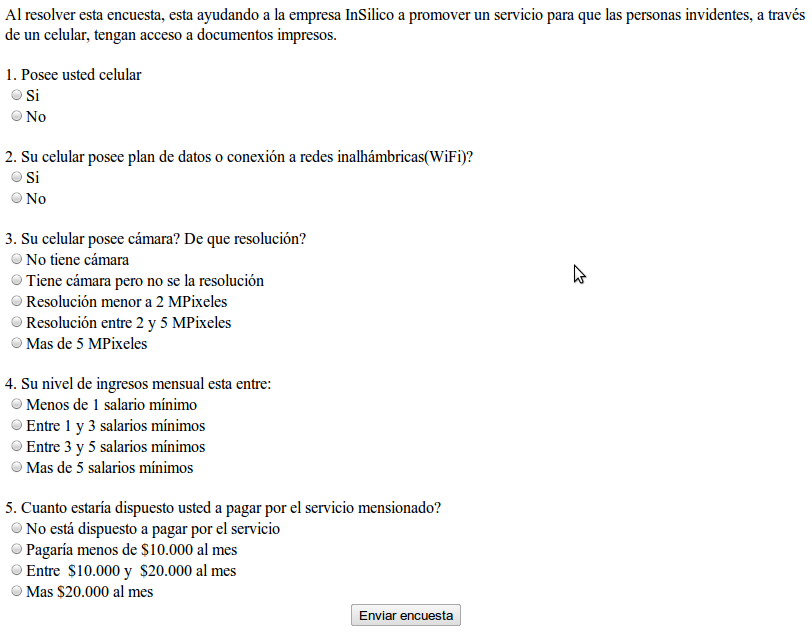
\includegraphics[width=12cm]{img/encuesta.png}
	\end{center}
	\caption{Instrumento de medición de la demanda}
	\label{fig:encuesta}
	\end{figure}
	
	\subsection{Técnica de Proyección de mercado}
	Después de estimar los 7 factores que influyen en las técnicas de proyección de mercado y los 5 criterios de validación, se llegó a la conclusión que el modelo causal es el mas apropiado. Las razones para la decisión son:
	\begin{itemize}
		\item No se han encontrado servicios iguales al servicio prestado actualmente, y no se encuentran tampoco servicios similares en el país. Por tanto un análisis histórico pierde validez, y el análisis de series de tiempo no tiene la precisión adecuada.
		\item Se encuentran numerosas estadísticas de entidades fiables como el DANE y el INCI que permiten relacionar las variables del mercado. Y una vez se tienen modelos que permiten relacionar las variables se puede hacer análisis matemáticos sobre estas relaciones para encontrar parámetros óptimos. Ya sea para minimizar el error en los modelos o para optimizar la ganancia.
		\item Dado que existen fuentes secundarias confiables, el costo de la recolección de datos no será tan alto.
		\item Al revisar el estado del ciclo de vida en el que se encuentra el producto, en el cual aun no se posee experiencia, no se puede aplicar el método de pronósticos visionarios.
	\end{itemize}
	Dentro de los modelos causales, se plantea utilizar el método de regresión lineal para determinar los parámetros de la demanda $A_1$, $A_2$ y $A_3$. Y la regresión se realiza sobre los datos recolectados en la encuesta de intensión de compra presentada previamente.
	
	\clearpage
	
	\begin{center}
	\section{Estudio técnico}
	\end{center}
	
	\subsection{Ingeniería del proyecto}
	
	\subsubsection{Proceso de producción}
	Para este proyecto, se escogió un modelo de producción por proyecto en lugar de utilizar modelos de producción en serie o pedido, dado que se desea prestar un servicio. En el caso de este servicio, el producto debe estar listo antes de atender los pedidos, y por esta razón la producción por pedido es descartada como opción. En el caso de la producción en serie, se debe tener en cuenta que lo que se desea producir es el software que va a prestar el servicio, y por esta razón, solo se necesita producir un único producto; este único producto tendrá la capacidad de atender peticiones de muchos usuarios.

	\subsubsection{Efectos económicos de la ingeniería}
	En esta sección determinaremos el costo de la prestación del servicio. El costo variable de atender cada petición de servicio de los usuarios depende del costo del servicio de internet, y del costo de mantenimiento y operación de los equipos servidores.\newline
	Sea entonces $I_p$ el costo del servicio de internet de responder una petición $p$, y $S_p$ el costo del cómputo de la petición $p$. Entonces el costo total de responder la petición $p$ es denotado $C_p$ y se calcula como:
	\begin{equation}
		C_p = I_p + S_p
		\label{eq:opCost}
	\end{equation}
	Dado que los equipos no tendrán la misma carga todo el tiempo, sino que tendrán momentos de horas pico y de baja carga, se asume el modelo general de ingeniería para estos procesos en el que la carga se modela como $y=\sin(x)$ en el intervalo $[0,\frac{\pi}{2}]$, y se toma como valor promedio la integral de la función $y$ dividida entre el periodo; se a demostrado que independiente del periodo la función es $\frac{1}{\sqrt{2}}$. Lo que quiere decir que asumiendo este modelo y un uso eficiente de los recursos, se puede concluir que el porcentaje promedio de uso óptimo de la capacidad de prestación del servicio sin disminuir la calidad esta dado por:
	\[ \mu_p=\frac{1}{\pi}\int_0^{\frac{\pi}{2}}{\sin(x)dx} = \frac{1}{\sqrt{2}} = 70.71\% \]
	Para calcular $I_p$ y $S_p$, se asume que se conoce el costo del Internet en un mes $I_m$ y el del mantenimiento y operación de los servicios de cómputo por mes $S_m$. Este costo $S_m$ contendrá el costo de la energía eléctrica requerida por los equipos de cómputo, así como su mantenimiento y operación. Además se debe conocer el tiempo promedio que toma responder una solicitud $t_p$, donde $t_p$ se mide en milisegundos. Entonces, dado que un mes tiene aproximadamente $2.6 \times 10^9$ milisegundos, entonces $I_p$ y $S_p$ son:
	\begin{align}
		I_p &= \frac{1}{2.6 \times 10^9 \times \mu_p}I_m \\
		S_p &= \frac{1}{2.6 \times 10^9 \times \mu_p}S_m
	\end{align}

	\subsubsection{Masa crítica técnica}
	Recordemos las ecuaciones de masa crítica técnica:
	\[\frac{P_2}{P_1} = \frac{C_2}{C_1}^{-a} \]

	Donde $P$ es el costo unitario de la operación, $C$ es la capacidad de la planta en unidades de producto, $a$ es el factor de volumen.

	\[ \frac{Q_2}{Q_1} = \frac{C_2}{C_1}^{-b} \]

	Donde $Q$ es el costo de equipos por unidad de capacidad y $b$ es un factor de volumen.

	\[ \frac{I_2}{I_1} = \frac{C_2}{C_1}^{f} \]

	Donde $I$ es inversión total y $f$ es un factor de volumen. 
	
	Un factor de volumen es la capacidad máxima de alguna variable que tiene una planta en un momento determinado. Antes de hallar los coeficientes requeridos en la masa 

	\subsection{Elección entre alternativas tecnológicas}
	
	\subsubsection{Factores cualitativos}
	Para este proyecto, se puede considerar como la materia prima los computadores y otros equipos necesarios para prestar el servicio a los usuarios. Aunque no hay proveedores de computadores que fabriquen sus equipos en la ciudad de Pereira, si hay distribuidores en la ciudad de equipos de cómputo, así como personal con capacitación técnica para el mantenimiento de estos equipos. Esto por que en la ciudad existen empresas dedicadas a prestar servicios informáticos en las que se necesitan los mismos insumos tecnológicos que los que se necesitan para este proyecto.
	Por otro lado, los recursos humanos no son tan fáciles de conseguir en la ciudad, dado que el desarrollo de este tipo de aplicativos requiere profesionales con conocimientos científicos, en los temas de algoritmia e inteligencia artificial, así como una buena competencia en ciencias básicas. Por fortuna algunos profesionales de la universidad tecnológica de Pereira son competentes en estas áreas, y en la medida en que se necesiten mas profesionales con este tipo de conocimientos, se espera que la universidad se preocupe mas en graduar profesionales con estos perfiles. Ya que hasta el momento el perfil del ingeniero de sistemas en la ciudad es principalmente el de sacar egresados con conocimientos técnicos en configuración de redes, que es lo que hasta el momento ha requerido la industria local.
	
	\subsubsection{Factores cuantitativos}
	Para hacer el análisis cuantitativo se propone utilizar en método de Lange. Lo primero que se debe hacer en este caso es determinar cual es el costo operativo y la inversión inicial en función del costo operativo. El costo operativo $C_p$ esta dado en la ecuación \ref{eq:opCost}. Dado que la inversión inicial $I_0$ depende del equipo de computo a comprar, y el costo $S_p$ también depende del equipo entonces la inversión inicial en función del costo se podría definir como:
	\begin{equation}
		I_0(C_p) = K_sS_p = K_s((S_p+I_p) - I_p) = K_s(C_p - I_p)
		\label{eq:InvCost}
	\end{equation}
	Donde $K_s$ es una constante que relaciona el costo inicial de los equipos y con el costo de mantenimiento, tal que $K_s=\frac{I_0}{S_p}$. Entonces si $n$ es el número de meses que dura el proyecto, por Lange tenemos:
	\begin{align*}
		min\{D&=I_o(C)+nC\} \\
		\frac{dI_o}{dC}&=-n \\
		K_s &= -n
	\end{align*}
	
	\subsection{Valoración económica de las variables}
	Las inversiones en obra física se muestran en la tabla \ref{tb:invFisica}, se decidió que la planta de producción de software y de alojamiento de los equipos servidores caben en un lote de aproximadamente $100m^2$, de los que se toma como área de máquinas un área de $10m \times 10m = 100m^2$ del segundo piso de la planta, en el tercer y cuarto piso de la planta están los desarrolladores de software y en el primero está la oficina de atención al cliente con un patio para el perro guardián y un baño. Para los valores residuales se asume una depreciación lineal con una duración del proyecto de 5 años.

	Las inversiones en personal se muestran en la tabla \ref{tb:invPersonal}, se considero que el proyecto, al tener un alto porcentaje investigativo, necesita al menos dos analistas. Los tres programadores son necesarios para la programación del código y el mantenimiento y actualización del mismo durante los 5 años. La secretaria es necesaria para atender el teléfono y a los clientes institucionales.

	Las inversiones en maquinaria se muestran en la tabla \ref{tb:invMaquinaria}, los cálculos se hicieron teniendo en cuenta un proyecto de 5 años. Cada miembro del personal tendrá un computador, y habrá un servidor para prestar el servicio. El perro guardián esta en esta tabla ya que esta parece ser la única tabla en la que tiene sentido ponerlo. Toda la maquinaria es necesaria para el correcto funcionamiento del proyecto y por tanto se comprara al inicio del mismo. De igual manera, toda la maquinaria se tiene presupuestada para durar los 5 años que dura el proyecto y por tanto se venderá cuando termine el mismo \footnote{Por esta razón no están las tablas calendario de inversiones e ingreso por ventas}.
	
	Las inversiones en materiales se muestran en la tabla \ref{tb:invMateriales}, los cálculos se hicieron teniendo en cuenta el personal y los requerimientos de la prestación del servicio.

	Las inversiones en insumos se muestran en la tabla \ref{tb:invInsumos}. Se calculo que los dispositivos utilizaran 1 kWh durante todo el año, los demás insumos se calcularon teniendo en cuenta el numero de personal. Las sillas y las mesas se clasificaron como insumos ya que se considero que esta era la categoría más lógica para estos elementos.
	
	\begin{table}
		\caption{Inversiones en obra física}
		\begin{tabular}{ | p{3cm} | p{1cm} | p{2.5cm} | p{2.5cm} | p{1cm} | p{2.2cm} | }
		\hline
		Item & Cant. & Costo unit. & Costo total & Vida útil & Valor residual \\
		\hline					
		Lote & $100m^2$ & \$100.000 & \$10.000.000 & N/A & \$10.000.000 \\
		\hline					
		Planta & 1 & \$200.000.000 & \$200.000.000 & 20 años & \$150.000.000 \\
		\hline
		Caseta del perro & 1 & \$200.000 & \$200.000 & 10 años & \$100.000 \\ 
		\hline
		Cercos & $400m$ & \$5.000 & \$2.000.000 & 10 años & \$1.000.000 \\
		\hline
		\end{tabular}
		\label{tb:invFisica}
	\end{table}

	\begin{table}
		\caption{Inversiones en maquinaria}
		\begin{tabular}{ | p{3cm} | p{1cm} | p{2.5cm} | p{2.5cm} | p{1cm} | p{2cm} | }
		\hline
		Maquina & Cant. & Valor unit. & Valor total & Vida útil & Valor residual \\
		\hline					
		Servidores & 1 & \$5.000.000 & \$5.000.000 & 7 años & \$2.142.857 \\
		\hline					
		Computadores & 5 & \$1.500.000 & \$7.500.000 & 5 años & \$0 \\
		\hline
		Impresoras & 1 & \$200.000 & \$200.000 & 5 años & \$0 \\ 
		\hline
		Routers & 1 & \$200.000 & \$200.000 & 5 años & \$0 \\
		\hline
		Ups & 2 & \$200.000 & \$400.000 & 10 años & \$200.000 \\
		\hline
		Perro & 1 & \$200.000 & \$200.000 & 10 años & \$100.000 \\
		\hline
		\end{tabular}
		\label{tb:invMaquinaria}
	\end{table}

	\begin{table}
		\caption{Inversiones en materiales}
		\begin{tabular}{ | p{3cm} | p{1.5cm} | p{1.5cm} | p{2cm} | p{2cm} | }
		\hline
		Material & Unidad & Cantidad & Costo unitario & Costo total \\
		\hline
		Tinta & unid. & 10 & \$50.000 & \$500.000 \\ 
		\hline					
		Papelería & hojas & 10000 & \$10 & \$100.000 \\
		\hline
		DVDs & unid. & 100 & \$1.000 & \$100.000 \\
		\hline
		USBs & unid. & 6 & \$50.000 & \$300.000 \\
		\hline
		\end{tabular}
		\label{tb:invMateriales}
	\end{table}

	\begin{table}
		\caption{Inversiones en personal}
		\begin{tabular}{ | p{3cm} | p{2cm} | p{2cm} | p{2cm} | }
		\hline
		Cargo & Numero & Rem. unit. & Rem. total \\
		\hline
		Analista & 2 & \$2.500.000 & \$60.000.000 \\
		\hline					
		Programador & 3 & \$1.200.000 & \$43.200.000 \\
		\hline
		Secretaria & 1 & \$800.000 & \$9.600.000 \\
		\hline
		\end{tabular}
		\label{tb:invPersonal}
	\end{table}

	\begin{table}
		\caption{Inversiones en insumos}
		\begin{tabular}{ | p{2.5cm} | p{1.5cm} | p{1.5cm} | p{2cm} | p{2cm} | }
		\hline
		Insumo & Unidad & Cantidad & Costo unitario & Costo total \\
		\hline					
		Energía & kWh & 8760 & \$250 & \$2.190.000 \\
		\hline					
		Agua potable & $m^{3}$ & 1825 & \$2.000 & \$3.650.000 \\
		\hline
		Papel h. & rollos & 50 & \$1.000 & \$50.000 \\
		\hline
		Mesas & unid. & 6 & \$150.000 & \$900.000 \\
		\hline
		Sillas & unid. & 5 & \$50.000 & \$250.000 \\
		\hline
		\end{tabular}
		\label{tb:invInsumos}
	\end{table}
		
	\subsection{Decisiones de tamaño}
	Suponiendo que se tienen U usuarios potencial, y que el tiempo de respuesta de una petición es $t_p$, y que cada usuario envía una petición en promedio cada $t_u$, se calcula la cantidad de usuarios que puede atender un servidor $U_s$ como:
  
	\begin{equation}
	U_s = \frac{t_u}{t_p \times \mu_p} 
	\label{eq:capacidad}
	\end{equation}

	\begin{itemize}
	 \item Capacidad teórica: $U_s$
	 \item Capacidad máxima: $max(U, U_s)$
	 \item Capacidad normal: $min(U, U_s)$
	\end{itemize}
	
	\subsection{Decisiones de localización}
	Se decidió localizar el proyecto en la ciudad de Pereira, ya que los factores más relevantes para este proyecto se cumplen: 

	\begin{itemize}
	 \item Existe una gran cantidad de ingenieros de sistemas y cada semestre se gradúan muchos más.
	 \item Debido a la crisis económica y al alto desempleo los costos de los terrenos han bajado, igual que el costo de construcción.
	 \item Hay una buena disponibilidad de internet, con varios proveedores potenciales, y también de agua y electricidad.
	\end{itemize}
 , 
	
	
	
	\clearpage

	\begin{center}
	\section{Consideraciones adicionales}
	\end{center}

	El proyecto que se describe en este documento es muy acorde a los planes de desarrollo consultados, pero, especialmente, a los objetivos del milenio acordados por los 192 países miembros de las Naciones Unidas. Dichos objetivos no solo son mencionados en todos los planes de desarrollo, sino que son base fundamental de los mismos. El objetivo del milenio más relacionado con nuestro proyecto es el 2do: lograr la enseñanza primaria universal. Este objetivo no puede llevarse a cabo si los niños invidentes en los lugares más alejados no tienen acceso a información escrita, algo que pensamos podemos ayudar a solucionar con este proyecto.
	El proyecto también apunta al mejoramiento de la calidad de vida de las personas invidentes, al darles
	acceso al conocimiento que se encuentra en textos impresos. Las personas invidentes necesitan no solo
	poder comunicarse entre ellos, sino poderse comunicar con el resto de personas. Es por esto que el sistema
	de escritura tradicional Braille se desea remplazar lentamente con alternativas de alta tecnología
	que les permita a las personas invidentes gozar de una mayor inclusión en la sociedad, conseguir empleos
	y tener cada vez menos restricciones por su limitación.
	
	\clearpage
	\begin{center}
	\section{Bibliografía}
	\end{center}
	AGRAWAL, Mudit y DOERMANN, David. Voronoi++: A Dynamic Page Segmentation approach based on Voronoi and Docstrum features. INTERNATIONAL CONFERENCE ON DOCUMENT ANALYSIS AND RECOGNITION. (10: 26-29, julio, 2009: Barcelona, Spain). Memorias, 2009. p. 1011-1015
	
	O'GORMAN Lawrence. The Document Spectrum for Page Layout Analysis. \underline{En}: IEEE Transactions on Pattern Analysis And Machine Intelligence. Noviembre, 1993. vol. 15, no. 11, p. 1162-1173
	
	BREUEL, Thomas. The OCRopus Open Source OCR System. DOCUMENT RECOGNITION AND RETRIVAL. (15: 29-31, febrero, 2008: San Jose, Estados Unidos). Memorias, 2008, p. 68-150
	
	SHAFAITA Faisal; KEYSERSA, Daniel y BREUEL, Thomas. Efficient Implementation of Local Adaptative Thersholding Techniques Using Integral Images. DOCUMENT RECOGNITION AND RETRIVAL. (15: 29-31, febrero, 2008: San Jose, Estados Unidos). Memorias, 2008, p. 61-67
	
	MAO Song; AZRIEL, Rosenfelda y KANUNGOB, Tapas. Document structure analysis algorithms: A literature survey. DOCUMENT RECOGNITION AND RETRIVAL. (10: enero, 2003: San Jose, Estados Unidos). Memorias, 2003, p. 197-207
	
	SHAFAITA Faisal; KEYSERSA, Daniel y BREUEL, Thomas. Performance Evaluation and Benchmarking of Six-Page segmentation Algorithms. \underline{En}: IEEE Transactions on Pattern Analysis And Machine Intelligence. Junio, 2008. vol. 30, no. 6, p. 941-954
	
	KISE, Koichi; SATO Akinori y MATSUMOTO, Keinosuke. Document Image Segmentation as Selection of Voronoi Edges. IEEE COMPUTER SOCIETY: CONFERENCE ON COMPUTER VISION AND PATTERN RECOGNITION (66: 17-19, junio, 1997: San Juan, Puerto Rico). Memorias, 1997, p. 32-39
	
	WONG, Kwan; CASEY, Richard y WAHL, Friedrich. Document Analysis System. \underline{En}: IBM Journal of Research and Development. Noviembre, 1982. vol. 26, no. 6, p. 647-656
	
	Ray Smith. An Overview of the Tesseract OCR Engine. IEEE COMPUTER SOCIETY: INTERNATIONAL CONFERENCE ON DOCUMENT ANALYSIS AND RECOGNITION (9: 23-26, septiembre, 2007: Curitiba, Paraná, Brazil). Memorias, 2007, p. 629-633
	
	ZHOU, Steven; SYED, Gilani y WINKLER, Stefan. Open Source OCR Framework Using Mobile Devices. MULTIMEDIA ON MOBILE DEVICES (1: 28-29 enero, 2008: San Jose, California, Estados Unidos). Memorias, 2008, vol. 6821, p. 682104.1-682104.6
	
	SENDA, Shuji, et al. Camera-Typing Interface for Ubiquitous Information Services. IEEE ANNUAL CONFERENCE ON PERVASIVE COMPUTING AND COMMUNICATIONS (2: 14-17, marzo, 2004: Orlando, Florida, Estados Unidos). Memorias, 2004, p. 366-372
	
	SMITH, Ray. Progress in Camera-Based Document Image Analysis. INTERNATIONAL CONFERENCE ON DOCUMENT ANALYSIS AND RECOGNITION (7: 3-6, agosto, 2003: Edimburgo, Escocia). Memorias, 2003, p. 606-617
	
	HU, Ming-Kuei. Visual pattern recognition by moment invariants. \underline{En}: IRE Transactions on Information Theory. Febrero, 1962, vol. 8, no. 2, p. 179-187
	
	SEUL, Machael , O'GORMAN Lawrence y SAMMON, Michael J. Practical Algorithms for Image Analysis. Nueva York: Cambridge University Press, 2000. 301 p.
	
	FLUSSER Jan, SUK, Tomas Suk y ZITOVA, Barbara. Moments and Moment Invariants in Pattern Recognition. Sussex, Reino Unido: Jhon Wiley \& Sons Ltd, 2009. 291 p.
	
	ALPAYDIN, Ethem. Introduction to Machine Learning. Estados Unidos: MIT Press, 2004. 415 p.
	
	CHERIET, Mohamed; KHARMA, Nawwaf y LIU Cheng-Lin. Character recognition systems: Guide for students and practitioners. New Jersey, Estados Unidos: Jhon Wiley \& Sons Ltd, 2007. 326 p.
	
	GUERRA, John Alexis; ZUNIGA, Maria Fernanda y RESTREPO, Felipe. Proyecto Iris. Trabajo de grado Ingeniero de Sistemas y Computación, Pereira: Universidad Tecnologia de Pereira, 2004
	
	MUÑOZ, Pablo Andrés. Máquinas de aprendizaje para reconocimiento de caracteres manuscritos. Tesis de Maestría en Ingeniería Eléctrica. Pereira: Universidad Tecnologica de Pereira, 2005
	
	RINCÓN, Jaime; LOAIZA, Johan Eric. Reconocimiento de palabras aisladas mediante redes neuronales sobre FPGA. Trabajo de grado Ingeniero Electricista. Pereira: Universidad Tecnologia de Pereira, 2008
	
	VALENCIA, Joan Mauricio; ABRIL Mauricio. Registro de transeúntes en tiempo real utilizando un sistema de visión artificial sobre un ambiente controlado. Trabajo de grado Ingeniero Electricista. Pereira: Universidad Tecnologia de Pereira, 2007
	
	ALVAREZ, Lorena. Acondicionamiento de Señales Bioeléctricas. Trabajo de grado Ingeniero Electricista. Pereira: Universidad Tecnologia de Pereira, 2007
	
	\clearpage
\end{document}
